% ============================================================
%  CHAPITRE 5 — SPRINT 3 : RAPPORTS, DIAGNOSTIC IA ET RENDEZ-VOUS
% ============================================================
\chapter{Sprint 3 : Rapports de Symptômes, Diagnostic IA et Rendez-vous}

\chapintro{Ce sprint implémente la boucle de diagnostic préliminaire et de prise
de rendez-vous. Le client soumet ses symptômes, le service IA génère un diagnostic
structuré, le chef d'atelier le révise puis propose une plage, et le client réserve
son rendez-vous.}

\section{Introduction}

La valeur ajoutée centrale de MecaRage réside dans son module de diagnostic IA.
Le service exploite une architecture RAG (Retrieval-Augmented Generation) combinant
l'algorithme BM25 pour la recherche dans la base de connaissances mécanique
et le modèle \textbf{Ollama} (LLM local, open-source) pour la génération du diagnostic structuré.

\section{Identification du Backlog Sprint 3}

\begin{table}[H]
\centering
\caption{Backlog Sprint 3 --- Symptômes, IA et Rendez-vous}
\label{tab:backlog-s3}
\begin{tabularx}{\textwidth}{|l|X|l|c|}
\hline
\rowcolor{gray!20}
\textbf{ID} & \textbf{User Story} & \textbf{Priorité} & \textbf{SP} \\
\hline
US10 & Client~: soumettre une description textuelle des symptômes & \prio{H} & 5 \\[3pt]\hline
US11 & Système~: déclencher automatiquement le service IA (RAG + Ollama) & \prio{H} & 8 \\[3pt]\hline
US12 & ChefAtelier~: réviser le rapport et proposer une plage de RDV & \prio{H} & 5 \\[3pt]\hline
US13 & Client~: réserver un rendez-vous dans la plage proposée & \prio{H} & 3 \\[3pt]\hline
US14 & ChefAtelier~: approuver ou refuser le rendez-vous & \prio{H} & 3 \\[3pt]\hline
\multicolumn{3}{|r|}{\textbf{Total Sprint 3}} & \textbf{24 SP} \\
\hline
\end{tabularx}
\end{table}

\noindent\textbf{Tâches techniques~:}
\begin{enumerate}[noitemsep]
  \item Entités \texttt{SymptomReport} et \texttt{Appointment}.
  \item Service IA FastAPI~: architecture RAG BM25 + Ollama (LLM local), endpoint
    \texttt{POST /diagnose}.
  \item Commandes~: \texttt{CreateSymptomReportCommand},
    \texttt{AddChefFeedbackCommand}, \texttt{CreateAppointmentCommand},
    \texttt{ApproveAppointmentCommand}.
  \item Intégration \texttt{HttpClient} côté back-end vers le service IA.
  \item Notifications automatiques au chef à chaque nouveau rapport.
  \item Interface Angular~: formulaire de symptômes, inbox chef, calendrier.
\end{enumerate}

\section{Conception}

\subsection{Diagramme de cas d'utilisation --- Sprint 3}

\begin{figure}[H]
\centering
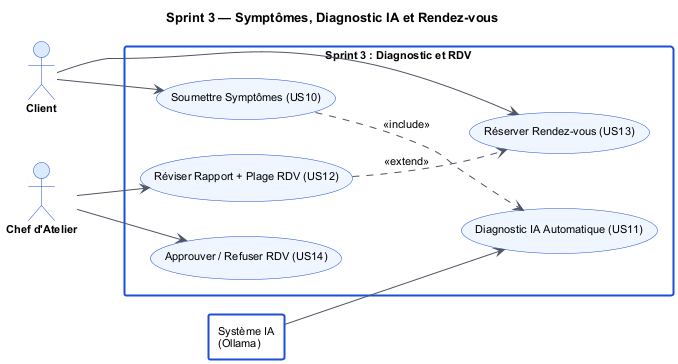
\includegraphics[width=0.85\textwidth]{diagrams/uc_s3.png}
\caption{Diagramme de cas d'utilisation --- Sprint 3}
\label{fig:uc-s3}
\end{figure}

\subsection{Pipeline du Diagnostic IA}

\begin{figure}[H]
\centering
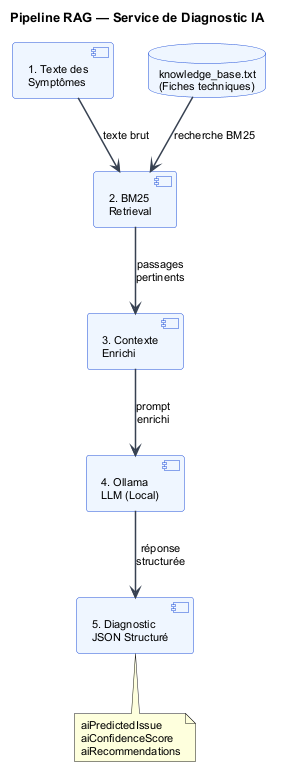
\includegraphics[width=0.85\textwidth]{diagrams/rag_pipeline.png}
\caption{Pipeline RAG --- Service de diagnostic IA}
\label{fig:rag-pipeline}
\end{figure}

\subsection{Diagramme de classes --- Sprint 3}

\begin{figure}[H]
\centering
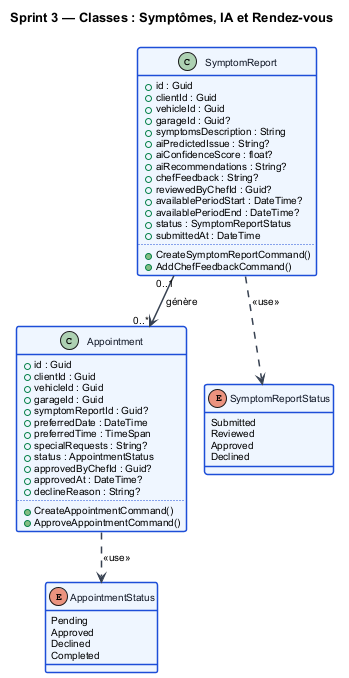
\includegraphics[width=\textwidth,height=0.62\textheight,keepaspectratio]{diagrams/class_s3.png}
\caption{Diagramme de classes --- Sprint 3 (Symptômes, IA et Rendez-vous)}
\label{fig:class-s3}
\end{figure}

\subsection{Diagramme de séquence}

\subsubsection*{SC5 --- Soumission de Symptômes et Diagnostic IA (US10+US11) :
fonctionnalité principale}

\noindent Le client soumet des symptômes, le système appelle le service IA, sauvegarde
le rapport enrichi, et notifie le chef d'atelier.

\begin{sidewaysfigure}[p]
\centering
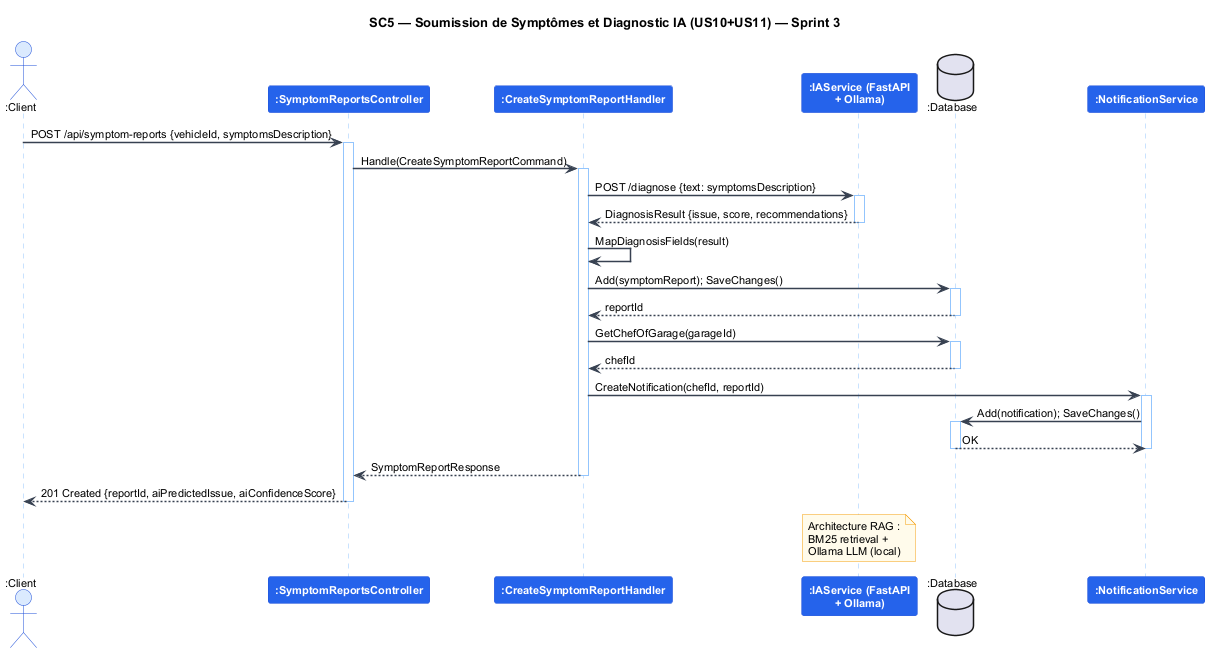
\includegraphics[width=0.92\textheight,keepaspectratio]{diagrams/seq_s3_symptom.png}
\caption{Diagramme de séquence SC5 --- Soumission de Symptômes et Diagnostic IA}
\label{fig:seq-s3-symptom}
\end{sidewaysfigure}

\section{Conclusion}

Le Sprint 3 a réalisé la première boucle de valeur visible par le client~: soumettre
des symptômes, recevoir un diagnostic IA instantané avec score de confiance, obtenir
une plage de rendez-vous proposée par le chef, et être notifié de sa confirmation.
L'approbation d'un rendez-vous déclenche automatiquement, via MediatR, la création
du traceur de cycle de vie de l'intervention.
